\documentclass[tikz,border=2mm]{standalone}
\usepackage{tikz}
\usetikzlibrary{shapes.geometric,arrows.meta,positioning,fit,patterns,calc,decorations.pathreplacing}

\begin{document}
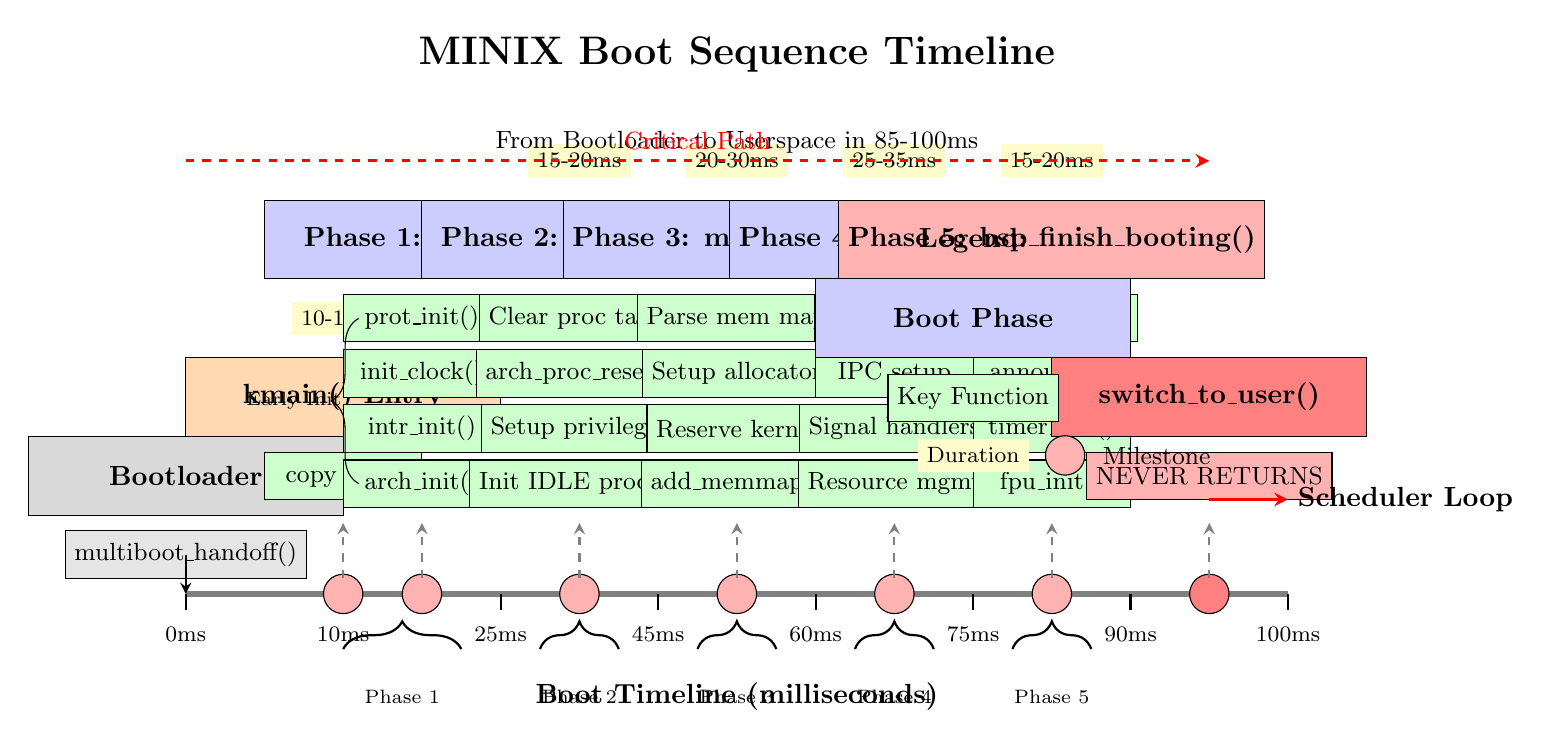
\begin{tikzpicture}[
    phase/.style={rectangle,draw,fill=blue!20,minimum width=4cm,minimum height=1cm,font=\bfseries},
    milestone/.style={circle,draw,fill=red!30,minimum size=0.5cm},
    function/.style={rectangle,draw,fill=green!20,minimum width=2cm,minimum height=0.6cm,font=\small},
    timing/.style={rectangle,draw=none,fill=yellow!20,minimum width=1cm,minimum height=0.4cm,font=\footnotesize},
    arrow/.style={->,>=stealth,thick},
    timeline/.style={line width=2pt,gray},
    brace/.style={decoration={brace,amplitude=10pt},decorate}
]

% Timeline
\draw[timeline] (0,0) -- (14,0);
\foreach \x/\t in {0/0ms,2/10ms,4/25ms,6/45ms,8/60ms,10/75ms,12/90ms,14/100ms} {
    \draw[thick] (\x,0) -- (\x,-0.2);
    \node[below] at (\x,-0.3) {\footnotesize\t};
}
\node[below,font=\bfseries] at (7,-1) {Boot Timeline (milliseconds)};

% Phase 0: Bootloader
\node[phase,fill=gray!30] at (0,1.5) {Bootloader};
\node[function,fill=gray!20] at (0,0.5) {multiboot\_handoff()};
\draw[arrow] (0,0.5) -- (0,0);

% Phase 1: kmain entry
\node[milestone] at (2,0) {};
\node[phase,fill=orange!30] at (2,2.5) {kmain() Entry};
\node[function] at (2,1.5) {copy kinfo};
\node[timing] at (2,3.5) {10-15ms};

% Phase 1.5: cstart (Early C init)
\node[milestone] at (3,0) {};
\node[phase] at (3,4.5) {Phase 1: cstart()};
\node[function] at (3,3.5) {prot\_init()};
\node[function] at (3,2.8) {init\_clock()};
\node[function] at (3,2.1) {intr\_init()};
\node[function] at (3,1.4) {arch\_init()};
\draw[brace] (2.2,1.4) -- (2.2,3.5);
\node[left,font=\scriptsize] at (2.1,2.45) {Early Init};

% Phase 2: Process management
\node[milestone] at (5,0) {};
\node[phase] at (5,4.5) {Phase 2: proc\_init()};
\node[function] at (5,3.5) {Clear proc table};
\node[function] at (5,2.8) {arch\_proc\_reset()};
\node[function] at (5,2.1) {Setup privileges};
\node[function] at (5,1.4) {Init IDLE process};
\node[timing] at (5,5.5) {15-20ms};

% Phase 3: Memory
\node[milestone] at (7,0) {};
\node[phase] at (7,4.5) {Phase 3: memory\_init()};
\node[function] at (7,3.5) {Parse mem map};
\node[function] at (7,2.8) {Setup allocator};
\node[function] at (7,2.1) {Reserve kernel};
\node[function] at (7,1.4) {add\_memmap()};
\node[timing] at (7,5.5) {20-30ms};

% Phase 4: System Services
\node[milestone] at (9,0) {};
\node[phase] at (9,4.5) {Phase 4: system\_init()};
\node[function] at (9,3.5) {Syscall table};
\node[function] at (9,2.8) {IPC setup};
\node[function] at (9,2.1) {Signal handlers};
\node[function] at (9,1.4) {Resource mgmt};
\node[timing] at (9,5.5) {25-35ms};

% Phase 5: Final Boot
\node[milestone] at (11,0) {};
\node[phase,fill=red!30] at (11,4.5) {Phase 5: bsp\_finish\_booting()};
\node[function] at (11,3.5) {cpu\_identify()};
\node[function] at (11,2.8) {announce()};
\node[function] at (11,2.1) {timer\_init()};
\node[function] at (11,1.4) {fpu\_init()};
\node[timing] at (11,5.5) {15-20ms};

% Switch to user (never returns)
\node[milestone,fill=red!50] at (13,0) {};
\node[phase,fill=red!50] at (13,2.5) {switch\_to\_user()};
\node[function,fill=red!30] at (13,1.5) {NEVER RETURNS};
\draw[arrow,very thick,red] (13,1.2) -- (14,1.2);
\node[right,font=\bfseries] at (14,1.2) {Scheduler Loop};

% Connection arrows
\foreach \x in {2,3,5,7,9,11,13} {
    \draw[arrow,gray,dashed] (\x,0.2) -- (\x,0.9);
}

% Phase grouping
\draw[brace,thick] (2,-0.7) -- (3.5,-0.7);
\node[below] at (2.75,-1.1) {\scriptsize Phase 1};
\draw[brace,thick] (4.5,-0.7) -- (5.5,-0.7);
\node[below] at (5,-1.1) {\scriptsize Phase 2};
\draw[brace,thick] (6.5,-0.7) -- (7.5,-0.7);
\node[below] at (7,-1.1) {\scriptsize Phase 3};
\draw[brace,thick] (8.5,-0.7) -- (9.5,-0.7);
\node[below] at (9,-1.1) {\scriptsize Phase 4};
\draw[brace,thick] (10.5,-0.7) -- (11.5,-0.7);
\node[below] at (11,-1.1) {\scriptsize Phase 5};

% Title and annotations
\node[above,font=\Large\bfseries] at (7,6.5) {MINIX Boot Sequence Timeline};
\node[below,font=\small] at (7,6) {From Bootloader to Userspace in 85-100ms};

% Critical path annotation
\draw[arrow,very thick,red,dashed] (0,5.5) -- node[above,sloped,font=\small] {Critical Path} (13,5.5);

% Legend
\node[phase,xshift=10cm,yshift=3.5cm] (legend1) {Boot Phase};
\node[function,below=0.2cm of legend1] (legend2) {Key Function};
\node[timing,below=0.2cm of legend2] (legend3) {Duration};
\node[milestone,right=0.2cm of legend3] (legend4) {};
\node[right=0.1cm of legend4,font=\small] {Milestone};
\node[above=0.2cm of legend1,font=\bfseries] {Legend:};

\end{tikzpicture}
\end{document}